\subsection{Bitcoin}
Currently the world's most used and most valued digital currency. Cryptocurrencies like Bitcoin dramatically fluctuate in value. In its peak Bitcoin was worth almost \$20000. During its peak Bitcoin was really popular among regular people, the media were talking about it, especially in the period of December-January 2018 as we can see in the graphs below.

\begin{figure}[H]
    \begin{left}
        \begin{minipage}{\linewidth}
            \begin{left}
                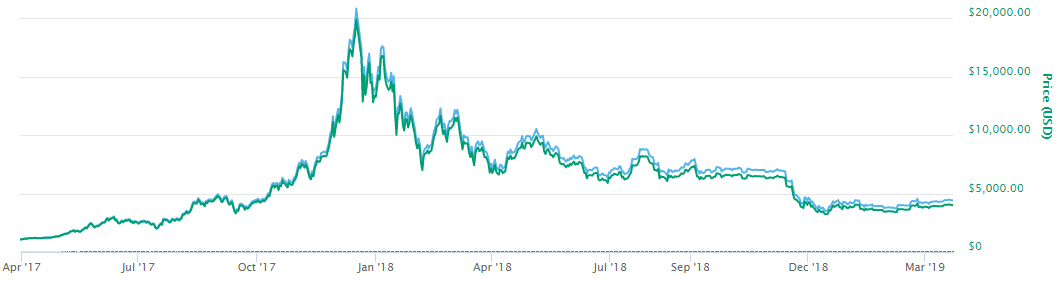
\includegraphics[width=\textwidth,keepaspectratio]{img/bitcoin_value.png}
                \caption{Bitcoin Value from April 2017 to March 2019}
                \label{obr 1.2.1}
            \end{left}
        \end{minipage}
    \end{left}
\end{figure}

\begin{figure}[H]
    \begin{left}
        \begin{minipage}{\linewidth}
            \begin{left}
                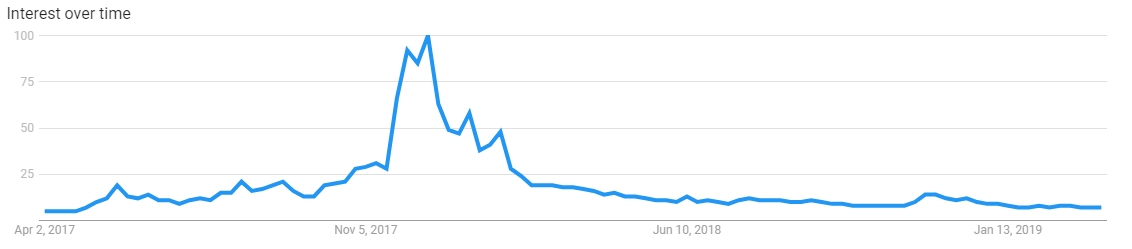
\includegraphics[width=\textwidth,keepaspectratio]{img/bitcoin_trends.png}
                \caption{Bitcoin Google search trends from April 2017 to March 2019}
                \label{obr 1.2.2}
            \end{left}
        \end{minipage}
    \end{left}
\end{figure}

Sending Bitcoin from one owner to another is called a transaction. The transaction has to be broadcasted to every peer in the network so they can update their copy of blockchain. After a broadcast was received, the network has to agree who has the latest version of blockchain with the new transaction. A node that has added a new block to the block chain is rewarded with a specific amount of Bitcoin. This process is called mining and it's the only way that new Bitcoins are created. The reward is getting smaller and will reach zero when the circulating supply of Bitcoins will be 21,000,000 BTC \cite{coinmarketcap_btc}. That reward started at 50 bitcoins per block. Every four years the protocol is adjusted, reducing the reward by half. One day the reward will be very small, but miners can also be rewarded by collecting fees volunteered by users that request transactions. This process takes around 10 minutes and it's called mining. A more detailed description of mining is available in section \hyperref[timestamping]{\textit{Time-Stamping schemes}}. 

\subsection{Etherium}
Ethereum was proposed in late 2013 and deployed in 2015 by Vitalik Buterin, a cryptocurrency researcher and programmer. It is an open blockchain platform that lets anyone build and use decentralised applications that run on blockchain technology. Like Bitcoin, no one controls or owns Ethereum – it is an open-source project \cite{eth_docs}.
The value of the Ethereum currency called Ether grew over 13 000\% in 2017, to over \$1400 and has fallen to \$130\cite{coinmarketcap}. Ether is the cryptocurrency that actually is the fuel, often referred to as a gas of this blockchain based platform. 
Ether is different from Bitcoin in several aspects. Time to add blocks to the blockchain is reduced from 10 minutes to 14-15 seconds. It uses the Ethash algorithm which reduces the advantage of specialized ASIC in mining. Transaction fees differ by computational complexity, bandwidth use and storage needs (in a system known as gas), while bitcoin transactions compete by means of transaction size, in bytes. Ethereum gas units each have a price that can be specified in a transaction. This is typically measured in Gwei. Bitcoin transactions usually have fees specified in satoshis per byte. Transaction fees are generally considerably lower for ether than for Bitcoin. In December 2017, the median transaction fee for ether corresponded to \$0.33, while for Bitcoin it corresponded to \$23. 

\subsection{Other}
CoinMarketCap lists more than 2000 cryptocurrencies while United Nations legal tender recognizes 180 currencies used worldwide \cite{List_of_circulating_currencies}. Other currencies are usually forked from Bitcoin Core, often referred to as AltCoins. AltCoin is an abbreviation of “Bitcoin alternative,” and  describes every single cryptocurrency except for Bitcoin. Altcoins are referred to as Bitcoin alternatives because, at least to some extent, most altcoins hope to either replace or improve upon at least one Bitcoin component. \cite{altcoin}. One of the signs of over saturation of the crypto market is the existence of parody coins like Dogecoin which was created as a joke currency. 

\subsection{Criticism}
Being decentralized and anonymous network open to everyone in the world, cryptocurrency faced criticism because of the lack of regulations, illegal activity and money laundering.

One of the early adopters of cryptocurrency were illegal markets as SilkRoad which accepted payments exclusively using Bitcoin. Estimated  turnover on the Silk Road anonymous online marketplace, the first to  support  Bitcoin  transactions  exclusively,  reached  \$15  million  per  year  just  one  year after it began operation. Any user holding bitcoins faces market risk via fluctuation in the exchange rate between bitcoin and other currencies. \cite{bitocin_doi}

A new type of malicious code became suddenly has become more and more popular. During one day ransomware WannaCry encrypted data on at least 75,000 computers in 99 countries. WannaCry encrypted all user data and demanded a ransom that could be only paid using  to decrypt the data. Russia's interior ministry, computers, hospitals in the United Kingdom, Telefonica in Spain, many schools in China were affected by this ransomware. The attack left hospitals and doctors unable to access patient data and led to the cancellation of operations and medical appointments. \cite{ransomware} 

Bitwise, a crypto-asset management firm, analyzed 81 exchanges, finding that 71 of them exhibited patterns that reflected artificial trading volume. One way to manufacture volume is via a technique called wash trading, in which someone simultaneously buys and sells the same asset. Although the exchanges in the study reported a combined \$6 billion in daily volume during four days this month, Bitwise determined that only \$273 million of it was real. \cite{bitwise_bitwise}